% !TEX root = main.tex
\section{量子化雑音の抑制手法とフィードフォワード型構成}
\label{sec:methods}

\subsection{既存の量子化雑音抑制手法}

分数分周比PLLの量子化雑音を抑制する手法は，大きく以下の3系統に整理できる．

\begin{enumerate}
  \item \textbf{デジタル-時間変換器(Digital-to-Time Converter, DTC)等によるノイズキャンセル：} MMDの制御列から期待される位相誤差を予測し，DTCで基準経路の時間をずらすことでキャンセルする．しかし，DTCが作る遅延は，温度や電圧，製造のばらつきにより変動しやすい．したがって，そのずれをキャリブレーションする回路が必要となる．また，キャリブレーションの収束には数十\,$\mu$s ~ 数\,msの時間がかかるうえ，PLLの出力周波数を切り替える度に再度キャリブレーションが必要になる(DTCの動作点が変わるため)．よって，特に頻繁に周波数が切り替わる設計の場合，PLLの出力品質が悪い時間が長いという欠点がある．
  \item \textbf{ノイズシェーピング周波数を上げる：} DSMの動作周波数(基本構成では基準周波数 $f_\text{REF}$ に一致)を高めることで，量子化雑音をより高域に押しやり，狭いループ帯域でも十分に除去できるようにする．しかし，そのためには高い基準周波数を持つ水晶発振器が必要となるため，必要コストが増大する．
  \item \textbf{等価FIRフィルタによる追加フィルタリング：} 同じPLLの出力成分に，遅延だけを変えた経路を複数用意する．各経路から出力された電流を(重みを変えて)足し合わせ平均化することで，主信号成分はそのままに雑音のみをキャンセルすることができる．これは，PLL出力それ自体は遅延に関係なく同じ値に収束するのに対し，量子化雑音は経路ごとにタイミングがずれるためである．しかし，遅延線が複雑になることや，消費電力が増大することが欠点である．
\end{enumerate}

第\ref{sec:pll-basics}節で述べた，フィードバックパスを分周器から高調波ミキサによる「引き算」に置き換える手法は，これら3系統とは異なる「新しいつまみ」として近年注目されており，他の手法と組み合わせることも可能である．ただし，この構成では補助PLLが新たに必要となるため，その補助VCOの消費電力や雑音をいかに抑えるかが課題となる．

\subsection{フィードフォワード(FF)型構成}

この補助VCOの雑音を軽減する手法として，Zhang et al.\cite{zhang_ffnc_2025}は，電圧領域のフィードフォワード雑音キャンセル(Feed-Forward Noise Cancellation, FFNC)を提案している(図\ref{fig:ff-concept})．この手法は，補助PLL側のPD出力(＝補助VCOの位相雑音の情報を含む信号)を，そのまま主ループのPD出力に加算するというものである．補助PLLにおいては，補助VCOの雑音はフィードバックパスに入る．それに対し，主ループでは基準側に入る．この入力経路の違いにより，2つを足し合わせることでノイズを打ち消すことができるのである．この手法は，補助PLLの雑音を打ち消すために高速な遅延線(VCDL)を用いる必要がなく，消費電力を抑えられるという利点がある．

\begin{figure}[H]
  \centering
  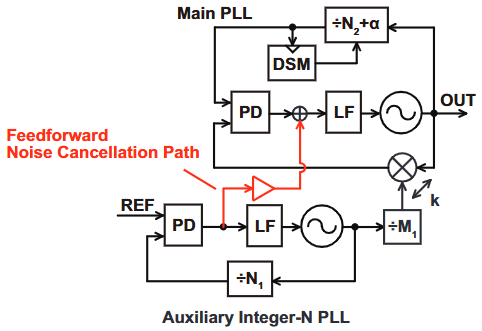
\includegraphics[keepaspectratio,width=0.85\columnwidth]{fig/fig_6_5.png}
  \caption{フィードフォワード雑音キャンセルの基本概念(本文Fig.\,6.5，\cite{osada_thesis})．補助PLLのPD出力を，電圧のまま主ループのPD出力に足し込むことで，高速な遅延線(VCDL)を使わずに補助VCOの雑音成分を打ち消す(\cite{zhang_ffnc_2025}, \cite{osada_thesis})．}
  \label{fig:ff-concept}
\end{figure}
